\documentclass{article}

\usepackage[letterpaper]{geometry}
\usepackage{tgpagella}
\usepackage{amsmath}
\usepackage{amssymb}
\usepackage{amsthm}
\usepackage{tikz}
\usepackage{minted}
\usepackage{physics}
\usepackage{siunitx}
\usepackage{gnuplot-lua-tikz}

\sisetup{detect-all}
\newtheorem{plm}{Problem}
\renewcommand*{\proofname}{Solution}

\title{4750 HW 4}
\author{Duncan Wilkie}
\date{28 October 2022}

\begin{document}

\maketitle

\begin{plm}[Standard Quantum Limit]
  Consider a simple Michelson interferometer to measure gravitational waves, with a ``DC'' readout (that is, not using an RF readout with sidebands,
  and not at the absolutely dark or absolutely bright fringe).
  \begin{enumerate}
  \item Assuming an operating point with output power $P_{out} \neq 0$, calculate the sensitivity of the photodiode power to the gravitational wave
    $h = \delta L / L$ (in other words, calculate $(dP_{out}/dh)$) as a function of the input power $P_{in}$.
  \item (Optional) The average number of photons arriving to a photodetector per unit time is $\bar{n} = P_{out} / (\hbar\omega) = \lambda P_{out} / (hc)$,
    where $\lambda$ is the laser wavelength and $h$ is Planck's constant.
    However, the actual number of photons will fluctuate due to their quantum nature, with a Gaussian distribution if $\bar{n}\gg 1$: this is ``shot noise.''
    Prove that these fluctuations are read as a noise in the GW readout with a frequency-independent amplitude spectral density
    \[
      h_{shot}(f) = \frac{1}{L}\sqrt{\frac{hc\lambda}{P_{in}}}.
    \]
  \item The average number of photons arriving at each end mirror is $(P_{in} / 2)/(\hbar\omega)$, and will push the mirror with radiation pressure.
    However, that power will also fluctuate, and that will be read as ``radiation pressure'' noise at the GW readout.
    Prove that at frequencies well above the suspended pendulum frequency, the noise in the readout will be
    \[
      h_{rp}(f) = \frac{1}{mf^{2}L}\sqrt{\frac{hP_{in}}{\pi^{2}c\lambda}}.
    \]
  \item (Optional) Plot the quadrature sum of the shot noise and radiation pressure noise $h = \sqrt{h_{shot}^{2} + h_{rp}^{2}}$ for \SI{40}{kg} mirrors,
    $\lambda = \SI{1064}{nm}$, and $L = \SI{4}{km}$ for three different input powers: \SI{40}{W}, \SI{40}{kW}, and \SI{40}{MW},
    for frequencies between \SI{0.1}{Hz} and \SI{1}{kHz} (assuming the pendulums are very, very long, with resonance frequencies below \SI{0.1}{Hz}).
    At what frequencies do each of the sums have their minimum value, and what is the minimum value?
  \item Using the expressions in previous parts, prove that the minimum value of the total quantum noise $h = \sqrt{h_{shot}^{2} + h_{rp}^{2}}$
    for any given input power (this is the ``standard quantum limit'') is independent of the input power or the operating point, and is given by
    \[
      h_{SQL} = \frac{1}{\pi fL}\sqrt{\frac{\hbar}{m}}.
    \]
  \end{enumerate}
\end{plm}

\begin{proof}
  For the first part,
  \[
    \dv{P_{out}}{h} = \dv{P_{out}}{\delta L}\dv{\delta L}{dh} = \dv{\delta L}\qty[P_{in}\sin^{2}(k\delta L)]\dv{h}\qty[hL]
    = kP_{in}L\sin(2k\delta L).
  \]
  Skipping the second, we assume the number of photons arriving at the end mirrors also has $\bar{n} \gg 1$, and so is Gaussian.
  A Gaussian distribution with mean $(P_{in} / 2) / (\hbar\omega)$
  Shot-type noise has variance equal to the average number of arriving photons, so the error in the momentum is
  \[
    \sqrt{\frac{P_{in}}{2\hbar\omega}}.
  \]
  Each photon carries linear momentum $h\lambda$; this translates to an error in the average force (as it has units momentum over time) of
  \[
    h\lambda\sqrt{\frac{P_{in}}{2\hbar\omega}}.
  \]
  At frequencies well above the suspended pendulum frequency, the system is well-modeled by a driven simple pendulum

  We can plot the expressions with gnuplot:
  \inputminted{gnuplot}{p1.gp}
  This produces the following:
  \begin{center}
    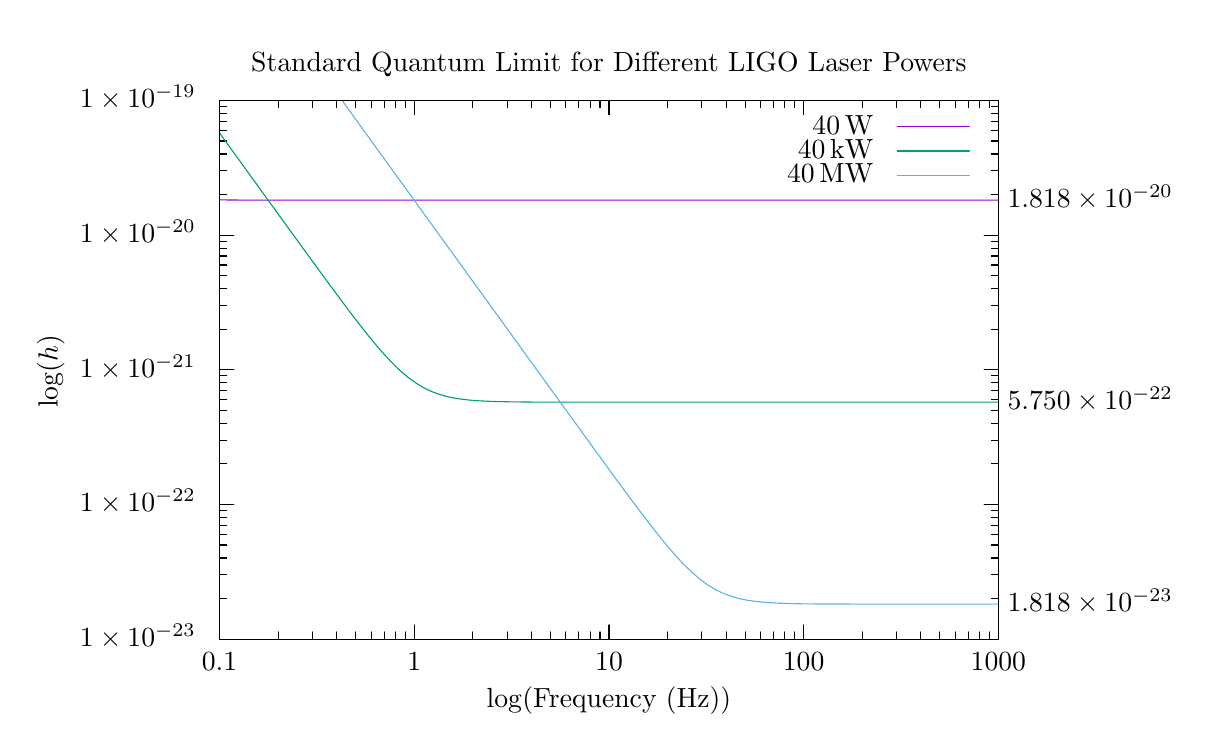
\begin{tikzpicture}[gnuplot]
%% generated with GNUPLOT 5.4p4 (Lua 5.3; terminal rev. Jun 2020, script rev. 115)
%% Thu 03 Nov 2022 10:39:51 PM CDT
\path (0.000,0.000) rectangle (12.500,8.750);
\gpcolor{color=gp lt color border}
\gpsetlinetype{gp lt border}
\gpsetdashtype{gp dt solid}
\gpsetlinewidth{1.00}
\draw[gp path] (2.056,0.985)--(2.236,0.985);
\draw[gp path] (11.947,0.985)--(11.767,0.985);
\node[gp node right] at (1.872,0.985) {$1\times10^{-23}$};
\draw[gp path] (2.056,1.500)--(2.146,1.500);
\draw[gp path] (11.947,1.500)--(11.857,1.500);
\draw[gp path] (2.056,1.801)--(2.146,1.801);
\draw[gp path] (11.947,1.801)--(11.857,1.801);
\draw[gp path] (2.056,2.015)--(2.146,2.015);
\draw[gp path] (11.947,2.015)--(11.857,2.015);
\draw[gp path] (2.056,2.180)--(2.146,2.180);
\draw[gp path] (11.947,2.180)--(11.857,2.180);
\draw[gp path] (2.056,2.316)--(2.146,2.316);
\draw[gp path] (11.947,2.316)--(11.857,2.316);
\draw[gp path] (2.056,2.430)--(2.146,2.430);
\draw[gp path] (11.947,2.430)--(11.857,2.430);
\draw[gp path] (2.056,2.529)--(2.146,2.529);
\draw[gp path] (11.947,2.529)--(11.857,2.529);
\draw[gp path] (2.056,2.617)--(2.146,2.617);
\draw[gp path] (11.947,2.617)--(11.857,2.617);
\draw[gp path] (2.056,2.695)--(2.236,2.695);
\draw[gp path] (11.947,2.695)--(11.767,2.695);
\node[gp node right] at (1.872,2.695) {$1\times10^{-22}$};
\draw[gp path] (2.056,3.210)--(2.146,3.210);
\draw[gp path] (11.947,3.210)--(11.857,3.210);
\draw[gp path] (2.056,3.511)--(2.146,3.511);
\draw[gp path] (11.947,3.511)--(11.857,3.511);
\draw[gp path] (2.056,3.725)--(2.146,3.725);
\draw[gp path] (11.947,3.725)--(11.857,3.725);
\draw[gp path] (2.056,3.890)--(2.146,3.890);
\draw[gp path] (11.947,3.890)--(11.857,3.890);
\draw[gp path] (2.056,4.026)--(2.146,4.026);
\draw[gp path] (11.947,4.026)--(11.857,4.026);
\draw[gp path] (2.056,4.140)--(2.146,4.140);
\draw[gp path] (11.947,4.140)--(11.857,4.140);
\draw[gp path] (2.056,4.239)--(2.146,4.239);
\draw[gp path] (11.947,4.239)--(11.857,4.239);
\draw[gp path] (2.056,4.327)--(2.146,4.327);
\draw[gp path] (11.947,4.327)--(11.857,4.327);
\draw[gp path] (2.056,4.405)--(2.236,4.405);
\draw[gp path] (11.947,4.405)--(11.767,4.405);
\node[gp node right] at (1.872,4.405) {$1\times10^{-21}$};
\draw[gp path] (2.056,4.920)--(2.146,4.920);
\draw[gp path] (11.947,4.920)--(11.857,4.920);
\draw[gp path] (2.056,5.221)--(2.146,5.221);
\draw[gp path] (11.947,5.221)--(11.857,5.221);
\draw[gp path] (2.056,5.435)--(2.146,5.435);
\draw[gp path] (11.947,5.435)--(11.857,5.435);
\draw[gp path] (2.056,5.600)--(2.146,5.600);
\draw[gp path] (11.947,5.600)--(11.857,5.600);
\draw[gp path] (2.056,5.736)--(2.146,5.736);
\draw[gp path] (11.947,5.736)--(11.857,5.736);
\draw[gp path] (2.056,5.850)--(2.146,5.850);
\draw[gp path] (11.947,5.850)--(11.857,5.850);
\draw[gp path] (2.056,5.949)--(2.146,5.949);
\draw[gp path] (11.947,5.949)--(11.857,5.949);
\draw[gp path] (2.056,6.037)--(2.146,6.037);
\draw[gp path] (11.947,6.037)--(11.857,6.037);
\draw[gp path] (2.056,6.115)--(2.236,6.115);
\draw[gp path] (11.947,6.115)--(11.767,6.115);
\node[gp node right] at (1.872,6.115) {$1\times10^{-20}$};
\draw[gp path] (2.056,6.630)--(2.146,6.630);
\draw[gp path] (11.947,6.630)--(11.857,6.630);
\draw[gp path] (2.056,6.931)--(2.146,6.931);
\draw[gp path] (11.947,6.931)--(11.857,6.931);
\draw[gp path] (2.056,7.145)--(2.146,7.145);
\draw[gp path] (11.947,7.145)--(11.857,7.145);
\draw[gp path] (2.056,7.310)--(2.146,7.310);
\draw[gp path] (11.947,7.310)--(11.857,7.310);
\draw[gp path] (2.056,7.446)--(2.146,7.446);
\draw[gp path] (11.947,7.446)--(11.857,7.446);
\draw[gp path] (2.056,7.560)--(2.146,7.560);
\draw[gp path] (11.947,7.560)--(11.857,7.560);
\draw[gp path] (2.056,7.659)--(2.146,7.659);
\draw[gp path] (11.947,7.659)--(11.857,7.659);
\draw[gp path] (2.056,7.747)--(2.146,7.747);
\draw[gp path] (11.947,7.747)--(11.857,7.747);
\draw[gp path] (2.056,7.825)--(2.236,7.825);
\draw[gp path] (11.947,7.825)--(11.767,7.825);
\node[gp node right] at (1.872,7.825) {$1\times10^{-19}$};
\draw[gp path] (2.056,0.985)--(2.056,1.165);
\draw[gp path] (2.056,7.825)--(2.056,7.645);
\node[gp node center] at (2.056,0.677) {$0.1$};
\draw[gp path] (2.800,0.985)--(2.800,1.075);
\draw[gp path] (2.800,7.825)--(2.800,7.735);
\draw[gp path] (3.236,0.985)--(3.236,1.075);
\draw[gp path] (3.236,7.825)--(3.236,7.735);
\draw[gp path] (3.545,0.985)--(3.545,1.075);
\draw[gp path] (3.545,7.825)--(3.545,7.735);
\draw[gp path] (3.784,0.985)--(3.784,1.075);
\draw[gp path] (3.784,7.825)--(3.784,7.735);
\draw[gp path] (3.980,0.985)--(3.980,1.075);
\draw[gp path] (3.980,7.825)--(3.980,7.735);
\draw[gp path] (4.146,0.985)--(4.146,1.075);
\draw[gp path] (4.146,7.825)--(4.146,7.735);
\draw[gp path] (4.289,0.985)--(4.289,1.075);
\draw[gp path] (4.289,7.825)--(4.289,7.735);
\draw[gp path] (4.416,0.985)--(4.416,1.075);
\draw[gp path] (4.416,7.825)--(4.416,7.735);
\draw[gp path] (4.529,0.985)--(4.529,1.165);
\draw[gp path] (4.529,7.825)--(4.529,7.645);
\node[gp node center] at (4.529,0.677) {$1$};
\draw[gp path] (5.273,0.985)--(5.273,1.075);
\draw[gp path] (5.273,7.825)--(5.273,7.735);
\draw[gp path] (5.709,0.985)--(5.709,1.075);
\draw[gp path] (5.709,7.825)--(5.709,7.735);
\draw[gp path] (6.017,0.985)--(6.017,1.075);
\draw[gp path] (6.017,7.825)--(6.017,7.735);
\draw[gp path] (6.257,0.985)--(6.257,1.075);
\draw[gp path] (6.257,7.825)--(6.257,7.735);
\draw[gp path] (6.453,0.985)--(6.453,1.075);
\draw[gp path] (6.453,7.825)--(6.453,7.735);
\draw[gp path] (6.618,0.985)--(6.618,1.075);
\draw[gp path] (6.618,7.825)--(6.618,7.735);
\draw[gp path] (6.762,0.985)--(6.762,1.075);
\draw[gp path] (6.762,7.825)--(6.762,7.735);
\draw[gp path] (6.888,0.985)--(6.888,1.075);
\draw[gp path] (6.888,7.825)--(6.888,7.735);
\draw[gp path] (7.002,0.985)--(7.002,1.165);
\draw[gp path] (7.002,7.825)--(7.002,7.645);
\node[gp node center] at (7.002,0.677) {$10$};
\draw[gp path] (7.746,0.985)--(7.746,1.075);
\draw[gp path] (7.746,7.825)--(7.746,7.735);
\draw[gp path] (8.181,0.985)--(8.181,1.075);
\draw[gp path] (8.181,7.825)--(8.181,7.735);
\draw[gp path] (8.490,0.985)--(8.490,1.075);
\draw[gp path] (8.490,7.825)--(8.490,7.735);
\draw[gp path] (8.730,0.985)--(8.730,1.075);
\draw[gp path] (8.730,7.825)--(8.730,7.735);
\draw[gp path] (8.926,0.985)--(8.926,1.075);
\draw[gp path] (8.926,7.825)--(8.926,7.735);
\draw[gp path] (9.091,0.985)--(9.091,1.075);
\draw[gp path] (9.091,7.825)--(9.091,7.735);
\draw[gp path] (9.235,0.985)--(9.235,1.075);
\draw[gp path] (9.235,7.825)--(9.235,7.735);
\draw[gp path] (9.361,0.985)--(9.361,1.075);
\draw[gp path] (9.361,7.825)--(9.361,7.735);
\draw[gp path] (9.474,0.985)--(9.474,1.165);
\draw[gp path] (9.474,7.825)--(9.474,7.645);
\node[gp node center] at (9.474,0.677) {$100$};
\draw[gp path] (10.219,0.985)--(10.219,1.075);
\draw[gp path] (10.219,7.825)--(10.219,7.735);
\draw[gp path] (10.654,0.985)--(10.654,1.075);
\draw[gp path] (10.654,7.825)--(10.654,7.735);
\draw[gp path] (10.963,0.985)--(10.963,1.075);
\draw[gp path] (10.963,7.825)--(10.963,7.735);
\draw[gp path] (11.203,0.985)--(11.203,1.075);
\draw[gp path] (11.203,7.825)--(11.203,7.735);
\draw[gp path] (11.398,0.985)--(11.398,1.075);
\draw[gp path] (11.398,7.825)--(11.398,7.735);
\draw[gp path] (11.564,0.985)--(11.564,1.075);
\draw[gp path] (11.564,7.825)--(11.564,7.735);
\draw[gp path] (11.707,0.985)--(11.707,1.075);
\draw[gp path] (11.707,7.825)--(11.707,7.735);
\draw[gp path] (11.834,0.985)--(11.834,1.075);
\draw[gp path] (11.834,7.825)--(11.834,7.735);
\draw[gp path] (11.947,0.985)--(11.947,1.165);
\draw[gp path] (11.947,7.825)--(11.947,7.645);
\node[gp node center] at (11.947,0.677) {$1000$};
\draw[gp path] (2.056,7.825)--(2.056,0.985)--(11.947,0.985)--(11.947,7.825)--cycle;
\node[gp node left] at (11.947,6.559) {\SI{1.818e-20}{}};
\node[gp node left] at (11.947,3.994) {\SI{5.750e-22}{}};
\node[gp node left] at (11.947,1.429) {\SI{1.818e-23}{}};
\node[gp node center,rotate=-270] at (-0.076,4.405) {$\log(h)$};
\node[gp node center] at (7.001,0.215) {$\log(\textrm{Frequency (Hz)})$};
\node[gp node right] at (10.479,7.491) {\SI{40}{W}};
\gpcolor{rgb color={0.580,0.000,0.827}}
\draw[gp path] (10.663,7.491)--(11.579,7.491);
\draw[gp path] (2.056,6.563)--(2.156,6.562)--(2.256,6.561)--(2.356,6.560)--(2.456,6.560)%
  --(2.556,6.560)--(2.655,6.559)--(2.755,6.559)--(2.855,6.559)--(2.955,6.559)--(3.055,6.559)%
  --(3.155,6.559)--(3.255,6.559)--(3.355,6.559)--(3.455,6.559)--(3.555,6.559)--(3.655,6.559)%
  --(3.754,6.559)--(3.854,6.559)--(3.954,6.559)--(4.054,6.559)--(4.154,6.559)--(4.254,6.559)%
  --(4.354,6.559)--(4.454,6.559)--(4.554,6.559)--(4.654,6.559)--(4.754,6.559)--(4.853,6.559)%
  --(4.953,6.559)--(5.053,6.559)--(5.153,6.559)--(5.253,6.559)--(5.353,6.559)--(5.453,6.559)%
  --(5.553,6.559)--(5.653,6.559)--(5.753,6.559)--(5.853,6.559)--(5.952,6.559)--(6.052,6.559)%
  --(6.152,6.559)--(6.252,6.559)--(6.352,6.559)--(6.452,6.559)--(6.552,6.559)--(6.652,6.559)%
  --(6.752,6.559)--(6.852,6.559)--(6.952,6.559)--(7.051,6.559)--(7.151,6.559)--(7.251,6.559)%
  --(7.351,6.559)--(7.451,6.559)--(7.551,6.559)--(7.651,6.559)--(7.751,6.559)--(7.851,6.559)%
  --(7.951,6.559)--(8.051,6.559)--(8.150,6.559)--(8.250,6.559)--(8.350,6.559)--(8.450,6.559)%
  --(8.550,6.559)--(8.650,6.559)--(8.750,6.559)--(8.850,6.559)--(8.950,6.559)--(9.050,6.559)%
  --(9.150,6.559)--(9.249,6.559)--(9.349,6.559)--(9.449,6.559)--(9.549,6.559)--(9.649,6.559)%
  --(9.749,6.559)--(9.849,6.559)--(9.949,6.559)--(10.049,6.559)--(10.149,6.559)--(10.249,6.559)%
  --(10.348,6.559)--(10.448,6.559)--(10.548,6.559)--(10.648,6.559)--(10.748,6.559)--(10.848,6.559)%
  --(10.948,6.559)--(11.048,6.559)--(11.148,6.559)--(11.248,6.559)--(11.348,6.559)--(11.447,6.559)%
  --(11.547,6.559)--(11.647,6.559)--(11.747,6.559)--(11.847,6.559)--(11.947,6.559);
\gpcolor{color=gp lt color border}
\node[gp node right] at (10.479,7.183) {\SI{40}{kW}};
\gpcolor{rgb color={0.000,0.620,0.451}}
\draw[gp path] (10.663,7.183)--(11.579,7.183);
\draw[gp path] (2.056,7.412)--(2.156,7.274)--(2.256,7.136)--(2.356,6.998)--(2.456,6.859)%
  --(2.556,6.721)--(2.655,6.583)--(2.755,6.445)--(2.855,6.307)--(2.955,6.169)--(3.055,6.032)%
  --(3.155,5.894)--(3.255,5.757)--(3.355,5.620)--(3.455,5.484)--(3.555,5.349)--(3.655,5.215)%
  --(3.754,5.083)--(3.854,4.954)--(3.954,4.828)--(4.054,4.707)--(4.154,4.593)--(4.254,4.487)%
  --(4.354,4.390)--(4.454,4.306)--(4.554,4.234)--(4.654,4.174)--(4.754,4.127)--(4.853,4.091)%
  --(4.953,4.063)--(5.053,4.043)--(5.153,4.029)--(5.253,4.018)--(5.353,4.011)--(5.453,4.006)%
  --(5.553,4.002)--(5.653,4.000)--(5.753,3.998)--(5.853,3.997)--(5.952,3.996)--(6.052,3.995)%
  --(6.152,3.995)--(6.252,3.995)--(6.352,3.994)--(6.452,3.994)--(6.552,3.994)--(6.652,3.994)%
  --(6.752,3.994)--(6.852,3.994)--(6.952,3.994)--(7.051,3.994)--(7.151,3.994)--(7.251,3.994)%
  --(7.351,3.994)--(7.451,3.994)--(7.551,3.994)--(7.651,3.994)--(7.751,3.994)--(7.851,3.994)%
  --(7.951,3.994)--(8.051,3.994)--(8.150,3.994)--(8.250,3.994)--(8.350,3.994)--(8.450,3.994)%
  --(8.550,3.994)--(8.650,3.994)--(8.750,3.994)--(8.850,3.994)--(8.950,3.994)--(9.050,3.994)%
  --(9.150,3.994)--(9.249,3.994)--(9.349,3.994)--(9.449,3.994)--(9.549,3.994)--(9.649,3.994)%
  --(9.749,3.994)--(9.849,3.994)--(9.949,3.994)--(10.049,3.994)--(10.149,3.994)--(10.249,3.994)%
  --(10.348,3.994)--(10.448,3.994)--(10.548,3.994)--(10.648,3.994)--(10.748,3.994)--(10.848,3.994)%
  --(10.948,3.994)--(11.048,3.994)--(11.148,3.994)--(11.248,3.994)--(11.348,3.994)--(11.447,3.994)%
  --(11.547,3.994)--(11.647,3.994)--(11.747,3.994)--(11.847,3.994)--(11.947,3.994);
\gpcolor{color=gp lt color border}
\node[gp node right] at (10.479,6.875) {\SI{40}{MW}};
\gpcolor{rgb color={0.337,0.706,0.914}}
\draw[gp path] (10.663,6.875)--(11.579,6.875);
\draw[gp path] (3.612,7.825)--(3.655,7.766)--(3.754,7.628)--(3.854,7.490)--(3.954,7.352)%
  --(4.054,7.213)--(4.154,7.075)--(4.254,6.937)--(4.354,6.799)--(4.454,6.661)--(4.554,6.522)%
  --(4.654,6.384)--(4.754,6.246)--(4.853,6.108)--(4.953,5.970)--(5.053,5.832)--(5.153,5.693)%
  --(5.253,5.555)--(5.353,5.417)--(5.453,5.279)--(5.553,5.141)--(5.653,5.002)--(5.753,4.864)%
  --(5.853,4.726)--(5.952,4.588)--(6.052,4.450)--(6.152,4.312)--(6.252,4.174)--(6.352,4.036)%
  --(6.452,3.897)--(6.552,3.760)--(6.652,3.622)--(6.752,3.484)--(6.852,3.346)--(6.952,3.209)%
  --(7.051,3.072)--(7.151,2.936)--(7.251,2.801)--(7.351,2.667)--(7.451,2.535)--(7.551,2.405)%
  --(7.651,2.279)--(7.751,2.157)--(7.851,2.042)--(7.951,1.934)--(8.051,1.837)--(8.150,1.751)%
  --(8.250,1.677)--(8.350,1.616)--(8.450,1.567)--(8.550,1.530)--(8.650,1.501)--(8.750,1.480)%
  --(8.850,1.465)--(8.950,1.454)--(9.050,1.447)--(9.150,1.441)--(9.249,1.438)--(9.349,1.435)%
  --(9.449,1.433)--(9.549,1.432)--(9.649,1.431)--(9.749,1.430)--(9.849,1.430)--(9.949,1.430)%
  --(10.049,1.430)--(10.149,1.429)--(10.249,1.429)--(10.348,1.429)--(10.448,1.429)--(10.548,1.429)%
  --(10.648,1.429)--(10.748,1.429)--(10.848,1.429)--(10.948,1.429)--(11.048,1.429)--(11.148,1.429)%
  --(11.248,1.429)--(11.348,1.429)--(11.447,1.429)--(11.547,1.429)--(11.647,1.429)--(11.747,1.429)%
  --(11.847,1.429)--(11.947,1.429);
\gpcolor{color=gp lt color border}
\draw[gp path] (2.056,7.825)--(2.056,0.985)--(11.947,0.985)--(11.947,7.825)--cycle;
\node[gp node center] at (7.001,8.287) {Standard Quantum Limit for Different LIGO Laser Powers};
%% coordinates of the plot area
\gpdefrectangularnode{gp plot 1}{\pgfpoint{2.056cm}{0.985cm}}{\pgfpoint{11.947cm}{7.825cm}}
\end{tikzpicture}
%% gnuplot variables

  \end{center}

  I wrote function optimization via bisection and central difference in Scheme for an old statistical mechanics assignment;
  I played around with that to see if there was variation in the flat parts,
  but the derivative appears to be \textit{zero} there to up to IEEE double-precision.
  I indicated the values of the functions at $\SI{1000}{Hz}$ on the graph; as the function appears otherwise monotonic,
  that is likely the minimum.

 % TODO: minimize
\end{proof}

\newpage
\begin{plm}
  Consider the feedback loop used in LIGO to keep the detector operating, with the signal at the antisymmetric port linear in $\Delta L$.
  For this, the difference in arm length needs to be controlled to have small fluctuations near the operation point:
  we call this the ``DARM loop.''
  A simple approximation of the loop is shown in the figure below.
  $\Delta L_{ext}$ represents the external disturbances to the arm length difference
  (due to the seismic noise, thermal noise, and gravitational waves), $e_{D}$ is the (digital) ``error'' signal (with units of digital ``counts'')
  we measure at the antisymmetric port, used to generate a control signal $c_{D}$ that pushes on one or both the end test masses to keep
  $\Delta l$ small.
  \[
    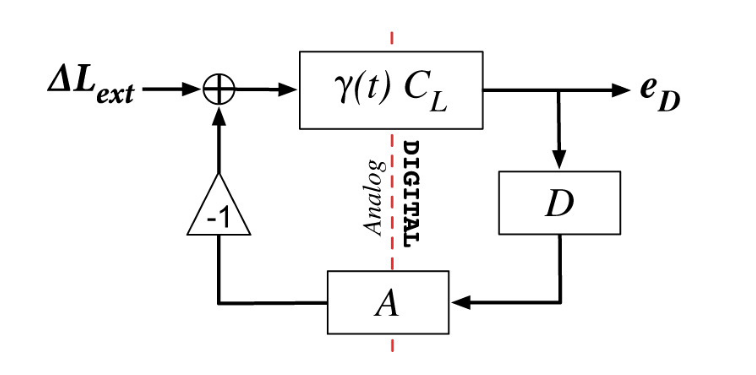
\includegraphics[scale=0.25]{loop.png}
  \]
  $C_{L}$ is the sensing function of the dual-recycled Fabry-Perot Michelson interferometer,
  which is approximated by a simple ``cavity pole'' transfer function and a constant gain $\gamma = \SI{500}{ct/nm}$:
  \[
    C(f) = \frac{\tilde{e}_{D}}{\Delta\tilde{L}} = \frac{\SI{500}{ct/nm}}{1 + if/(\SI{350}{Hz})}
  \]
  (in reality, the gain of the sensing function varies due to alignment fluctuations, and we track it by injecting ``calibration lines'').
  The actuation function is the response of the pendulum, which will approximate that of a simple pendulum
  \[
    A(f) = \frac{\Delta\tilde{L}}{\tilde{c}_{D}} = \frac{\SI{1}{pm/ct}}{1 - (f / \SI{0.7}{Hz})^{2} - i(f / \SI{0.7}{Hz})}
  \]
  (We can use a simple pendulum approximation when we push the test mass from the reaction chain at the bottom of the quadruple pendulum,
  using an electrostatic actuator, and we also need to track its gain with calibration lines.
  We also need to push on upper masses, which complicates the actual actuation function.)
  \begin{enumerate}
  \item Design a simple digital controller (try first a constant) that results in an open loop gain with unity gain frequency at \SI{100}{Hz},
    and plot the open-loop gain and the closed-loop gain for frequencies between \SI{0.1}{Hz} and \SI{1}{kHz}.
  \item Prove that we can produce a ``calibrated strain'' as $\tilde{h} = (\tilde{e}_{D}/C_{L}(f) + A(f)\tilde{e}_{C})/L$.
  \item (Optional) Using the seismic excitation you used in Homework 3 and the digital controller of part (a),
    plot the amplitude spectral density of the residual displacement $(\Delta L_{ext} - \Delta L_{ctrl}),$
    and calculate the residual rms as a fraction of the laser wavelength (\SI{1064}{nm}).
  \item (Optional) There is sensor noise (shot noise at the photodiode) added to the signal of the optical sensor.
    Assuming we have an ADC for the photocurrent with gain $\SI{10}{V}/\SI{16384}{cts}$, and \SI{800}{W} on the beamsplitter,
    plot the amplitude spectral density of calibrated strain limited by shot noise.
  \end{enumerate}
\end{plm}

\begin{proof}
  We seek a $\tilde{D}(f)$ such that
  \[
    |\tilde{G}(f)| = |\tilde{A}(f)\tilde{D}(f)\tilde{C}(f)| = 1
  \]
  at $f = \SI{100}{Hz}$.
  Taking the ansatz $\tilde{D}(f) = c$,
  \[
    |c| = \frac{1}{|\tilde{A}(f)\tilde{C}(f)|} = \frac{1}{\left|\frac{\SI{500}{ct/nm}}{1 + if/(\SI{350}{Hz})}
        \frac{\SI{1}{pm/ct}}{1 - (f/\SI{0.7}{Hz})^{2} - i(f / \SI{0.7}{Hz})}\right|}
  \]
  \[
    = \left|\frac{1 - (f / \SI{0.7}{Hz})^{2} - i(f / \SI{0.7}{Hz}) + if/(\SI{350}{Hz}) - if(f / \SI{0.7}{Hz})^{2}/(\SI{350}{Hz})
        + f^{2}/(\SI{245}{Hz})}{\SI{0.5}{m^{-1}}}\right|
  \]
  \[
    = \left| \frac{1 - i\frac{f^{3}}{\SI{172}{Hz}}+ f^{2}(\frac{1}{\SI{245}{Hz}} - \frac{1}{\SI{0.49}{Hz^{2}}})
      + if(\frac{1}{\SI{350}{Hz}} - \frac{1}{\SI{0.7}{Hz}})}{\SI{0.5}{m^{-1}}} \right|
    = \left| \SI{2}{m}\qty(1 - \frac{i}{\SI{172}{Hz}}f^{3} - {2.04}f^{2} - 1.43if) \right|
  \]
  Evaluating this at $f = \SI{100}{Hz}$, $|c| = 42500$.
  The open-loop gain is the expression $|G(f)|$ above, and the closed-loop gain is $H(f) = \frac{1}{1 + G(f)}$.
  Plotting with gnuplot,
  \begin{center}
    \inputminted{gnuplot}{p2.gp}
  \end{center}
  results in
  \begin{center}
    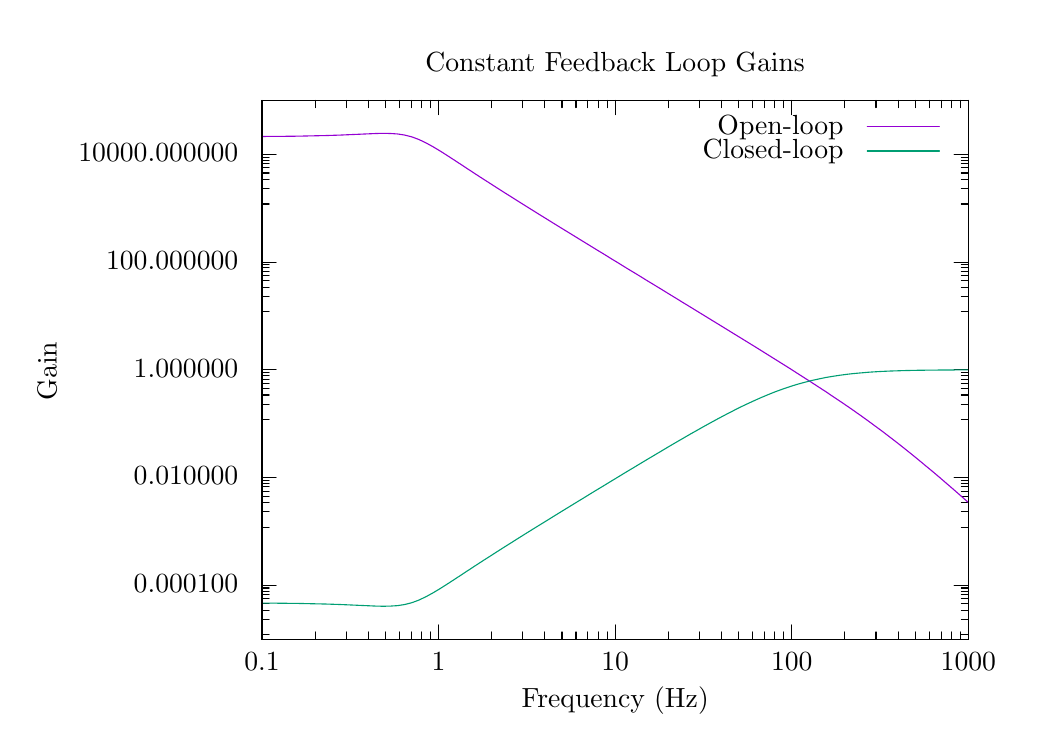
\begin{tikzpicture}[gnuplot]
%% generated with GNUPLOT 5.4p4 (Lua 5.3; terminal rev. Jun 2020, script rev. 115)
%% Fri 04 Nov 2022 11:03:05 PM CDT
\path (0.000,0.000) rectangle (12.500,8.750);
\gpcolor{color=gp lt color border}
\gpsetlinetype{gp lt border}
\gpsetdashtype{gp dt solid}
\gpsetlinewidth{1.00}
\draw[gp path] (2.976,1.039)--(3.066,1.039);
\draw[gp path] (11.947,1.039)--(11.857,1.039);
\draw[gp path] (2.976,1.232)--(3.066,1.232);
\draw[gp path] (11.947,1.232)--(11.857,1.232);
\draw[gp path] (2.976,1.349)--(3.066,1.349);
\draw[gp path] (11.947,1.349)--(11.857,1.349);
\draw[gp path] (2.976,1.432)--(3.066,1.432);
\draw[gp path] (11.947,1.432)--(11.857,1.432);
\draw[gp path] (2.976,1.497)--(3.066,1.497);
\draw[gp path] (11.947,1.497)--(11.857,1.497);
\draw[gp path] (2.976,1.550)--(3.066,1.550);
\draw[gp path] (11.947,1.550)--(11.857,1.550);
\draw[gp path] (2.976,1.595)--(3.066,1.595);
\draw[gp path] (11.947,1.595)--(11.857,1.595);
\draw[gp path] (2.976,1.634)--(3.066,1.634);
\draw[gp path] (11.947,1.634)--(11.857,1.634);
\draw[gp path] (2.976,1.669)--(3.156,1.669);
\draw[gp path] (11.947,1.669)--(11.767,1.669);
\node[gp node right] at (2.792,1.669) {0.000100};
\draw[gp path] (2.976,2.407)--(3.066,2.407);
\draw[gp path] (11.947,2.407)--(11.857,2.407);
\draw[gp path] (2.976,2.600)--(3.066,2.600);
\draw[gp path] (11.947,2.600)--(11.857,2.600);
\draw[gp path] (2.976,2.717)--(3.066,2.717);
\draw[gp path] (11.947,2.717)--(11.857,2.717);
\draw[gp path] (2.976,2.800)--(3.066,2.800);
\draw[gp path] (11.947,2.800)--(11.857,2.800);
\draw[gp path] (2.976,2.865)--(3.066,2.865);
\draw[gp path] (11.947,2.865)--(11.857,2.865);
\draw[gp path] (2.976,2.918)--(3.066,2.918);
\draw[gp path] (11.947,2.918)--(11.857,2.918);
\draw[gp path] (2.976,2.963)--(3.066,2.963);
\draw[gp path] (11.947,2.963)--(11.857,2.963);
\draw[gp path] (2.976,3.002)--(3.066,3.002);
\draw[gp path] (11.947,3.002)--(11.857,3.002);
\draw[gp path] (2.976,3.037)--(3.156,3.037);
\draw[gp path] (11.947,3.037)--(11.767,3.037);
\node[gp node right] at (2.792,3.037) {0.010000};
\draw[gp path] (2.976,3.775)--(3.066,3.775);
\draw[gp path] (11.947,3.775)--(11.857,3.775);
\draw[gp path] (2.976,3.968)--(3.066,3.968);
\draw[gp path] (11.947,3.968)--(11.857,3.968);
\draw[gp path] (2.976,4.085)--(3.066,4.085);
\draw[gp path] (11.947,4.085)--(11.857,4.085);
\draw[gp path] (2.976,4.168)--(3.066,4.168);
\draw[gp path] (11.947,4.168)--(11.857,4.168);
\draw[gp path] (2.976,4.233)--(3.066,4.233);
\draw[gp path] (11.947,4.233)--(11.857,4.233);
\draw[gp path] (2.976,4.286)--(3.066,4.286);
\draw[gp path] (11.947,4.286)--(11.857,4.286);
\draw[gp path] (2.976,4.331)--(3.066,4.331);
\draw[gp path] (11.947,4.331)--(11.857,4.331);
\draw[gp path] (2.976,4.370)--(3.066,4.370);
\draw[gp path] (11.947,4.370)--(11.857,4.370);
\draw[gp path] (2.976,4.405)--(3.156,4.405);
\draw[gp path] (11.947,4.405)--(11.767,4.405);
\node[gp node right] at (2.792,4.405) {1.000000};
\draw[gp path] (2.976,5.143)--(3.066,5.143);
\draw[gp path] (11.947,5.143)--(11.857,5.143);
\draw[gp path] (2.976,5.336)--(3.066,5.336);
\draw[gp path] (11.947,5.336)--(11.857,5.336);
\draw[gp path] (2.976,5.453)--(3.066,5.453);
\draw[gp path] (11.947,5.453)--(11.857,5.453);
\draw[gp path] (2.976,5.536)--(3.066,5.536);
\draw[gp path] (11.947,5.536)--(11.857,5.536);
\draw[gp path] (2.976,5.601)--(3.066,5.601);
\draw[gp path] (11.947,5.601)--(11.857,5.601);
\draw[gp path] (2.976,5.654)--(3.066,5.654);
\draw[gp path] (11.947,5.654)--(11.857,5.654);
\draw[gp path] (2.976,5.699)--(3.066,5.699);
\draw[gp path] (11.947,5.699)--(11.857,5.699);
\draw[gp path] (2.976,5.738)--(3.066,5.738);
\draw[gp path] (11.947,5.738)--(11.857,5.738);
\draw[gp path] (2.976,5.773)--(3.156,5.773);
\draw[gp path] (11.947,5.773)--(11.767,5.773);
\node[gp node right] at (2.792,5.773) {100.000000};
\draw[gp path] (2.976,6.511)--(3.066,6.511);
\draw[gp path] (11.947,6.511)--(11.857,6.511);
\draw[gp path] (2.976,6.704)--(3.066,6.704);
\draw[gp path] (11.947,6.704)--(11.857,6.704);
\draw[gp path] (2.976,6.821)--(3.066,6.821);
\draw[gp path] (11.947,6.821)--(11.857,6.821);
\draw[gp path] (2.976,6.904)--(3.066,6.904);
\draw[gp path] (11.947,6.904)--(11.857,6.904);
\draw[gp path] (2.976,6.969)--(3.066,6.969);
\draw[gp path] (11.947,6.969)--(11.857,6.969);
\draw[gp path] (2.976,7.022)--(3.066,7.022);
\draw[gp path] (11.947,7.022)--(11.857,7.022);
\draw[gp path] (2.976,7.067)--(3.066,7.067);
\draw[gp path] (11.947,7.067)--(11.857,7.067);
\draw[gp path] (2.976,7.106)--(3.066,7.106);
\draw[gp path] (11.947,7.106)--(11.857,7.106);
\draw[gp path] (2.976,7.141)--(3.156,7.141);
\draw[gp path] (11.947,7.141)--(11.767,7.141);
\node[gp node right] at (2.792,7.141) {10000.000000};
\draw[gp path] (2.976,0.985)--(2.976,1.165);
\draw[gp path] (2.976,7.825)--(2.976,7.645);
\node[gp node center] at (2.976,0.677) {$0.1$};
\draw[gp path] (3.651,0.985)--(3.651,1.075);
\draw[gp path] (3.651,7.825)--(3.651,7.735);
\draw[gp path] (4.046,0.985)--(4.046,1.075);
\draw[gp path] (4.046,7.825)--(4.046,7.735);
\draw[gp path] (4.326,0.985)--(4.326,1.075);
\draw[gp path] (4.326,7.825)--(4.326,7.735);
\draw[gp path] (4.544,0.985)--(4.544,1.075);
\draw[gp path] (4.544,7.825)--(4.544,7.735);
\draw[gp path] (4.721,0.985)--(4.721,1.075);
\draw[gp path] (4.721,7.825)--(4.721,7.735);
\draw[gp path] (4.871,0.985)--(4.871,1.075);
\draw[gp path] (4.871,7.825)--(4.871,7.735);
\draw[gp path] (5.001,0.985)--(5.001,1.075);
\draw[gp path] (5.001,7.825)--(5.001,7.735);
\draw[gp path] (5.116,0.985)--(5.116,1.075);
\draw[gp path] (5.116,7.825)--(5.116,7.735);
\draw[gp path] (5.219,0.985)--(5.219,1.165);
\draw[gp path] (5.219,7.825)--(5.219,7.645);
\node[gp node center] at (5.219,0.677) {$1$};
\draw[gp path] (5.894,0.985)--(5.894,1.075);
\draw[gp path] (5.894,7.825)--(5.894,7.735);
\draw[gp path] (6.289,0.985)--(6.289,1.075);
\draw[gp path] (6.289,7.825)--(6.289,7.735);
\draw[gp path] (6.569,0.985)--(6.569,1.075);
\draw[gp path] (6.569,7.825)--(6.569,7.735);
\draw[gp path] (6.786,0.985)--(6.786,1.075);
\draw[gp path] (6.786,7.825)--(6.786,7.735);
\draw[gp path] (6.964,0.985)--(6.964,1.075);
\draw[gp path] (6.964,7.825)--(6.964,7.735);
\draw[gp path] (7.114,0.985)--(7.114,1.075);
\draw[gp path] (7.114,7.825)--(7.114,7.735);
\draw[gp path] (7.244,0.985)--(7.244,1.075);
\draw[gp path] (7.244,7.825)--(7.244,7.735);
\draw[gp path] (7.359,0.985)--(7.359,1.075);
\draw[gp path] (7.359,7.825)--(7.359,7.735);
\draw[gp path] (7.462,0.985)--(7.462,1.165);
\draw[gp path] (7.462,7.825)--(7.462,7.645);
\node[gp node center] at (7.462,0.677) {$10$};
\draw[gp path] (8.137,0.985)--(8.137,1.075);
\draw[gp path] (8.137,7.825)--(8.137,7.735);
\draw[gp path] (8.532,0.985)--(8.532,1.075);
\draw[gp path] (8.532,7.825)--(8.532,7.735);
\draw[gp path] (8.812,0.985)--(8.812,1.075);
\draw[gp path] (8.812,7.825)--(8.812,7.735);
\draw[gp path] (9.029,0.985)--(9.029,1.075);
\draw[gp path] (9.029,7.825)--(9.029,7.735);
\draw[gp path] (9.207,0.985)--(9.207,1.075);
\draw[gp path] (9.207,7.825)--(9.207,7.735);
\draw[gp path] (9.357,0.985)--(9.357,1.075);
\draw[gp path] (9.357,7.825)--(9.357,7.735);
\draw[gp path] (9.487,0.985)--(9.487,1.075);
\draw[gp path] (9.487,7.825)--(9.487,7.735);
\draw[gp path] (9.602,0.985)--(9.602,1.075);
\draw[gp path] (9.602,7.825)--(9.602,7.735);
\draw[gp path] (9.704,0.985)--(9.704,1.165);
\draw[gp path] (9.704,7.825)--(9.704,7.645);
\node[gp node center] at (9.704,0.677) {$100$};
\draw[gp path] (10.379,0.985)--(10.379,1.075);
\draw[gp path] (10.379,7.825)--(10.379,7.735);
\draw[gp path] (10.774,0.985)--(10.774,1.075);
\draw[gp path] (10.774,7.825)--(10.774,7.735);
\draw[gp path] (11.055,0.985)--(11.055,1.075);
\draw[gp path] (11.055,7.825)--(11.055,7.735);
\draw[gp path] (11.272,0.985)--(11.272,1.075);
\draw[gp path] (11.272,7.825)--(11.272,7.735);
\draw[gp path] (11.449,0.985)--(11.449,1.075);
\draw[gp path] (11.449,7.825)--(11.449,7.735);
\draw[gp path] (11.600,0.985)--(11.600,1.075);
\draw[gp path] (11.600,7.825)--(11.600,7.735);
\draw[gp path] (11.730,0.985)--(11.730,1.075);
\draw[gp path] (11.730,7.825)--(11.730,7.735);
\draw[gp path] (11.844,0.985)--(11.844,1.075);
\draw[gp path] (11.844,7.825)--(11.844,7.735);
\draw[gp path] (11.947,0.985)--(11.947,1.165);
\draw[gp path] (11.947,7.825)--(11.947,7.645);
\node[gp node center] at (11.947,0.677) {$1000$};
\draw[gp path] (2.976,7.825)--(2.976,0.985)--(11.947,0.985)--(11.947,7.825)--cycle;
\node[gp node center,rotate=-270] at (0.292,4.405) {Gain};
\node[gp node center] at (7.461,0.215) {Frequency (Hz)};
\node[gp node right] at (10.479,7.491) {Open-loop};
\gpcolor{rgb color={0.580,0.000,0.827}}
\draw[gp path] (10.663,7.491)--(11.579,7.491);
\draw[gp path] (2.976,7.368)--(3.067,7.369)--(3.157,7.369)--(3.248,7.370)--(3.338,7.371)%
  --(3.429,7.372)--(3.520,7.374)--(3.610,7.376)--(3.701,7.378)--(3.792,7.380)--(3.882,7.383)%
  --(3.973,7.386)--(4.063,7.390)--(4.154,7.394)--(4.245,7.398)--(4.335,7.402)--(4.426,7.406)%
  --(4.516,7.408)--(4.607,7.406)--(4.698,7.400)--(4.788,7.386)--(4.879,7.363)--(4.970,7.329)%
  --(5.060,7.286)--(5.151,7.236)--(5.241,7.182)--(5.332,7.124)--(5.423,7.065)--(5.513,7.006)%
  --(5.604,6.946)--(5.694,6.887)--(5.785,6.828)--(5.876,6.770)--(5.966,6.712)--(6.057,6.654)%
  --(6.148,6.597)--(6.238,6.540)--(6.329,6.483)--(6.419,6.427)--(6.510,6.370)--(6.601,6.314)%
  --(6.691,6.258)--(6.782,6.202)--(6.872,6.147)--(6.963,6.091)--(7.054,6.035)--(7.144,5.980)%
  --(7.235,5.924)--(7.326,5.869)--(7.416,5.813)--(7.507,5.758)--(7.597,5.702)--(7.688,5.647)%
  --(7.779,5.592)--(7.869,5.536)--(7.960,5.481)--(8.051,5.426)--(8.141,5.370)--(8.232,5.315)%
  --(8.322,5.259)--(8.413,5.204)--(8.504,5.148)--(8.594,5.093)--(8.685,5.037)--(8.775,4.982)%
  --(8.866,4.926)--(8.957,4.870)--(9.047,4.815)--(9.138,4.759)--(9.229,4.703)--(9.319,4.647)%
  --(9.410,4.590)--(9.500,4.534)--(9.591,4.477)--(9.682,4.420)--(9.772,4.362)--(9.863,4.304)%
  --(9.953,4.246)--(10.044,4.187)--(10.135,4.128)--(10.225,4.067)--(10.316,4.006)--(10.407,3.945)%
  --(10.497,3.882)--(10.588,3.818)--(10.678,3.753)--(10.769,3.686)--(10.860,3.619)--(10.950,3.550)%
  --(11.041,3.480)--(11.131,3.409)--(11.222,3.336)--(11.313,3.262)--(11.403,3.187)--(11.494,3.112)%
  --(11.585,3.035)--(11.675,2.957)--(11.766,2.879)--(11.856,2.800)--(11.947,2.720);
\gpcolor{color=gp lt color border}
\node[gp node right] at (10.479,7.183) {Closed-loop};
\gpcolor{rgb color={0.000,0.620,0.451}}
\draw[gp path] (10.663,7.183)--(11.579,7.183);
\draw[gp path] (2.976,1.442)--(3.067,1.441)--(3.157,1.441)--(3.248,1.440)--(3.338,1.439)%
  --(3.429,1.438)--(3.520,1.436)--(3.610,1.434)--(3.701,1.432)--(3.792,1.430)--(3.882,1.427)%
  --(3.973,1.424)--(4.063,1.420)--(4.154,1.416)--(4.245,1.412)--(4.335,1.408)--(4.426,1.404)%
  --(4.516,1.402)--(4.607,1.404)--(4.698,1.410)--(4.788,1.424)--(4.879,1.447)--(4.970,1.481)%
  --(5.060,1.524)--(5.151,1.574)--(5.241,1.628)--(5.332,1.686)--(5.423,1.745)--(5.513,1.804)%
  --(5.604,1.864)--(5.694,1.923)--(5.785,1.982)--(5.876,2.040)--(5.966,2.098)--(6.057,2.156)%
  --(6.148,2.213)--(6.238,2.270)--(6.329,2.327)--(6.419,2.383)--(6.510,2.439)--(6.601,2.495)%
  --(6.691,2.551)--(6.782,2.607)--(6.872,2.662)--(6.963,2.718)--(7.054,2.773)--(7.144,2.829)%
  --(7.235,2.884)--(7.326,2.939)--(7.416,2.994)--(7.507,3.049)--(7.597,3.104)--(7.688,3.158)%
  --(7.779,3.213)--(7.869,3.267)--(7.960,3.321)--(8.051,3.375)--(8.141,3.429)--(8.232,3.482)%
  --(8.322,3.534)--(8.413,3.587)--(8.504,3.638)--(8.594,3.689)--(8.685,3.739)--(8.775,3.788)%
  --(8.866,3.836)--(8.957,3.883)--(9.047,3.929)--(9.138,3.972)--(9.229,4.014)--(9.319,4.054)%
  --(9.410,4.092)--(9.500,4.128)--(9.591,4.161)--(9.682,4.192)--(9.772,4.220)--(9.863,4.245)%
  --(9.953,4.268)--(10.044,4.288)--(10.135,4.307)--(10.225,4.322)--(10.316,4.336)--(10.407,4.348)%
  --(10.497,4.358)--(10.588,4.366)--(10.678,4.374)--(10.769,4.380)--(10.860,4.385)--(10.950,4.389)%
  --(11.041,4.392)--(11.131,4.395)--(11.222,4.397)--(11.313,4.399)--(11.403,4.400)--(11.494,4.401)%
  --(11.585,4.402)--(11.675,4.403)--(11.766,4.403)--(11.856,4.404)--(11.947,4.404);
\gpcolor{color=gp lt color border}
\draw[gp path] (2.976,7.825)--(2.976,0.985)--(11.947,0.985)--(11.947,7.825)--cycle;
\node[gp node center] at (7.461,8.287) {Constant Feedback Loop Gains};
%% coordinates of the plot area
\gpdefrectangularnode{gp plot 1}{\pgfpoint{2.976cm}{0.985cm}}{\pgfpoint{11.947cm}{7.825cm}}
\end{tikzpicture}

  \end{center}
\end{proof}

\begin{plm}
  Let's use a simple Michelson detector at the dark port using phase modulation of the input laser and an RF readout.
  \begin{enumerate}
  \item Consider the input laser modulated, and expanded using Bessel functions of the first kind
    \[
      E = E_{0}e^{i(\omega t + \Gamma \sin(\Omega t))} = E_{0}e^{i\omega t}\sum_{n = -\infty}^{\infty}J_{n}(\Gamma)e^{in\Omega t}
    \]
    Given an average arm length $L$, a time-independent macroscopic (Shnupp) arm length difference $\Delta L \gg \lambda$
    and a very small fluctuation in arm length difference $\delta L \ll \lambda$ from a dark operating point where $kL = n\pi$,
    calculate the output power to first order in $\delta L$.
  \item Assume we use a low-pass filter to eliminate terms oscillating with $2\Omega$ frequencies or higher,
    but keep terms oscillating with $\Omega$.
    Write down the output power as $P_{out} = P_{DC} + A\sin(\Omega t) + B\cos(\omega T)$ (again, to first order in $\delta L$).
  \item (Optional) What's the shot noise produced by the power on the photodiode?
    Consider the DC term and the oscillating terms.
  \item Now let's demodulate the signal.
    Assuming we convert the power in the photodiode into a voltage $V_{out} = \eta ZP_{out}$
    ($\eta$ is the quantum PD efficiency in \si{A/W}, $Z$ is impedance used in the readout in Ohms),
    calculate the demodulated signals $V_{Q} = V_{out}\sin(\Omega t + \phi)$ and $V_{I} = V_{out}\sin(\Omega t + \phi)$,
    where $\phi$ is a phase we will tune in the last part.
  \item Write down the expressions for the demodulated signals $V_{Q}, V_{I}$ after using another low-pass filter to eliminate terms
    oscillating at $n\Omega$.
  \item Find the phase $\phi$ that makes one of the demodulated signals zero, and the other proportional to $\delta L$:
    we can now read a GW signal with a simple Michelson operating at the (carrier) dark port!
  \end{enumerate}
\end{plm}

\begin{proof}
  Using $P = |E|^{2}$,
  \[
    P = E_{0}^{2}\left| \sum_{n = -\infty}^{\infty}J_{n}(\Gamma)e^{in\Omega t} \right|^{2}
  \]
  Asymptotically, $J_{n}(\Gamma) \to \frac{1}{(n + 1)!}\qty(\frac{\Gamma}{2})^{n}$ as $\Gamma \to 0$,
  so for larger $|n|$ the contribution of the term is smaller.
  Accordingly, we take only the carrier and the first sidebands.
  \[
    P = E_{0}^{2}\qty|J_{0}(\Gamma) + J_{1}(\Gamma)e^{i\Omega t} - J_{1}(\Gamma)e^{-i\Omega t}|^{2}
    = E_{0}^{2}\qty|J_{0}(\Gamma) + 2J_{1}(\Gamma)\cos(\Omega t)|^{2}
  \]
  \[
    = E_{0}^{2}\qty(J_{0}(\Gamma)^{2} + 4J_{0}(\Gamma)J_{1}(\Gamma)\cos(\Omega t) + 4J_{1}(\Gamma)^{2}\cos^{2}(\Omega t))
  \]
  Writing
\end{proof}

\begin{plm}
  Consider two mirrors with amplitude reflectivity and transmissivity $r_{1}, t_{1}, r_{2}, t_{2}$ at a fixed distance $L$,
  and an input electric field $E = E_{0}e^{i\omega t}$ traveling in the $z$-direction, perpendicular to the mirrors,
  incident at mirror 1 which is at $z = 0$.
  Assume the ``$+$'' side of the mirrors are the sides facing each other.
  \begin{enumerate}
  \item Follow the singe beam that is reflected from and transmitted through mirror 1:
    now there are two beams, one traveling forward in the cavity and another traveling back to the laser.
    The transmitted beam travels to mirror 2 (picking up a phase $e^{ikL}$) and is then reflected from and transmitted through mirror 2:
    now there are three beams: two traveling forward, one inside the cavity and one transmitted by the cavity,
    and two beams traveling back: the one promptly reflected by mirror 1 and the one reflected from mirror 2.
    The single beam reflected from mirror 2 is now reflected from and transmitted through mirror 2\ldots you get the idea.
    Draw several of these beams and the expression for the fields for each one on each side of the mirror, and write the total transmitted beam,
    the total reflected beam, and the total field traveling forward in the cavity as a sum of exponentials.
  \item Using the identity $\frac{1}{1 - x} = \sum_{n = 0}^{\infty}x^{n}$, obtain an expression for the total reflected beam,
    the total transmitted beam, and the total forward traveling beam in the cavity
    (compare these with the ones we derived in class using a steady state).
  \item Plot the amplitude and phase of the cavity transmissivity, gain, and reflectivity as a function of the variable $f - f_{0}$
    with $f_{0} = c / \lambda$ for $L = \SI{4}{km}$, $\lambda = \SI{1064}{nm}$, and $f - f_{0}$ between $\SI{-40}{kHz}$ and $\SI{40}{kHz}$.
  \end{enumerate}
\end{plm}

\end{document}
